\newpage
\section{Introduzione all'ottimizzazione matematica}

% Introduzione
\subsection{Introduzione}

Partiamo da un \hl{insieme di formule ed equazioni che modelleranno il problema}. Con questo modello proviamo a trovare una \hl{soluzione} al nostro problema \hl{attraverso algoritmi o risolutori}. L'output è una soluzione per il nostro modello da implementare nel mondo reale.


% Ingredienti principali
\subsection{Ingredienti principali}

Gli ingredienti principali sanno:

\begin{itemize}
	\item \textbf{dati} del problema
	\item variabili: dette anche var decisionali: scelte da fare in merito al problema. rappresentano quindi le scelte, quello su cui il decisore può intervenire
	\item vincoli: equazioni che definiscono i valori che le variabili possono assumere
	\item funzione obietivo: sarà una formula che rappresenta una misura di tipo quantitativo per capire quando è buona la soluzione che abbiamo ottenuto. quindi dovremo ottimizzare questo valore in base al contesto
\end{itemize}


Parleremo di \hl{programmazione lineare con modelli matematici} o relazioni lineari, dato che \hl{molti problemi reali si rifanno a modelli lineari}, per quanto essi possano essere complessi.


% Descrizione del problema
\subsection{Descrizione del problema}

Proviamo a risolvere un problema di mix di produzione, cioè un sistema con un impianto con 2 stabilimenti in cui:

\begin{enumerate}
	\item nel primo: diamo le materie prime e vengono realizzati i componenti in uscita
	\item nel secondo: diamo i componenti realizzati che vengono assemblati per creare il prodotto finito
	\end{enumerate}


\begin{figure}[H]
\centering
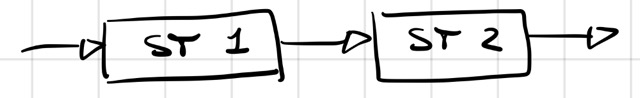
\includegraphics[scale=0.3]{st12.jpeg}
\caption{Catena tra i due stabilimenti} 
\label{st12}
\end{figure}


Supponendo di voler realizzare 2 prodotti A, B con un differente profitto. Determinare il \hl{mix di produzione}, cioè quante unità di A e B produrre la prossima settimana.
Saranno presenti dei \hl{vincoli} creati dalle risorse come i macchinari o gli addetti che potranno lavorare un numero di ore finito.


% Dati del problema
\subsection{Dati del problema}

\begin{itemize}
	\item ore di lavoro:

	\begin{table}[h!]
		\begin{center}
			\begin{tabular}{|c | c c c|} 
 				\hline
 				Stab & A & B & Addetti \\ [0.5ex]
 				\hline
	 			1 & 4 ore & 2 ore & 10 \\
 				2 & 2 ore & 4 ore & 10 \\
				\hline
			\end{tabular}
		\end{center}
		\caption{Tabella delle ore di lavoro}
		\label{taborelav}
	\end{table}

	\item ogni addetto lavora 40 ore/settimana
	
	\item profitto €/pallet:
	
	\begin{table}[h!]
		\begin{center}
			\begin{tabular}{| c c|} 
 				\hline
 				A & B \\ [0.5ex]
 				\hline
 				15k & 10k \\
				\hline
			\end{tabular}
		\end{center}
		\caption{Tabella del profitto €/pallet}
		\label{tabprof}
	\end{table}
	
	\item richiesta del prodotto nella prossima settimana:
	
	\begin{table}[h!]
		\begin{center}
			\begin{tabular}{| c c|} 
 				\hline
 				A & B \\ [0.5ex]
 				\hline
 				40 & 120 \\
				\hline
			\end{tabular}
		\end{center}
		\caption{Tabella del profitto euro/pallet}
		\label{tabprof}
	\end{table}

\end{itemize}


% Descrizione del problema con un modello matematico
\subsection{Descrizione del problema con un modello matematico}

Per \hl{effettuare una modellazione} faremo:

\begin{enumerate}
	\item \hl{identificare le variabili decisionali}:
		\begin{itemize}
			\item $x_A$: \# di pallet di prodotto A da realizzare
			\item $x_B$: \# di pallet di prodotto B da realizzare
		\end{itemize}
		
	\item \hl{definire la funzione obbiettivo (FO)}, per massimizzare il profitto

	\item \hl{definire i vincoli espressi come uguaglianza o disuguaglianza}
		\begin{itemize}
			\item vincolo 1: capacità produttiva dello stab 1 $4x_A+2x_B$ che non può superare $40*10$ cioè ore disponibili ogni settimana per un addetto * numero di addetti: $$4x_A+2x_B \leq 400$$
			\item vincolo 2: capacità produttiva dello stabilimento 2 $2x_A+4x_B$ che non può superare $40*10$ cioè ore disponibili ogni settimana per un addetto * numero di addetti: $$4x_A+2x_B \leq 400$$
			\item vincolo 3: vincolo sulla richiesta di A: $$x_A \leq 40$$
			\item vincolo 4: vincolo sulla richiesta di B: $$x_B \leq 120$$
			\item vincolo 5: vincolo di non-negatività: $$x_A, x_B \geq 0$$
		\end{itemize}
		
	
\end{enumerate}

	
	
Nella forma completa il \hl{modello complessivo} è:

$$MAX=z=15x_A+10x_B$$

sottoposto ai vincoli (sv):

\begin{itemize}
	\item $4x_A+2x_B \leq 400$
	\item $2x_A+4x_B \leq 400$
	\item $x_A \leq 40$
	\item $x_B \leq 120$
	\item $x_A, x_B \geq 0$
\end{itemize}


% Risolvere il modello matematico
\subsection{Risolvere il modello matematico}

\hl{Rappresentiamo sul piano cartesiano tutte le soluzioni ammissibili} cercando quella che massimizza il nostro risultato

Impostiamo delle rette per ogni vincolo:

\begin{itemize}
	\item presa $4x_A+2x_B \leq 400$ poniamo = 0, a turno, $x_A$ e $x_B$: (200, 100)
	\item presa $2x_A+4x_B \leq 400$ poniamo = 0, a turno, $x_A$ e $x_B$: (100, 200)
	\item presa $x_A \leq 40$: (40, 0)
	\item presa $x_B \leq 120$: (0, 120)
\end{itemize}


Avremo allora una \hl{regione ammissibile} dove valgono tutti i vincoli e nella quale dovrebbe essere presente la nostra soluzione ammissibile. Per trovare il punto che rende massima la funzione $z$ usiamo il \hl{metodo del gradiente}:

$$\nabla z = \left[\begin{array}{c}
	\dfrac{dz}{dx_A}\\
	\dfrac{dz}{dx_B}
\end{array}\right] = \left[\begin{array}{c}
	15\\
	10
\end{array}\right]
$$

dove $\nabla z$ sarà la massima crescita che viene rappresentata tramite (15, 10).

Tracciando una \hl{retta perpendicolare (curve di livello)} alla retta del gradiente avremo valori sempre buoni ma più bassi di quelli sul gradiente, a patto che siano validi. Troveremo in fine il punto massimo che consente di massimizzare, cioè il più estremo alla regione ammissibile sarà il nostro punto.

\hl{Seguendo la retta del gradiente troviamo che la soluzione ottimale} si trova nell'intersezione tra le rette del vincolo 2 con il 3: $x_A = 40$ $2*40+4X_B=400$ quindi $x_B=80$.

La soluzione ottimale sarà:

$$\begin{cases} 
    x_A = 40 \\ 
    2x_A+4x_B = 400
\end{cases}
\begin{cases} 
    x_A = 40 \\ 
    x_B = 80
\end{cases}$$


Si nota che lo stabilimento 2 viene saturato e quello 1 no, dal fatto che la soluzione giace sulla retta del vincolo per il quale si satura.


% Terminologia
\subsection{Terminologia}

Possiamo avere altre forme di modelli di PL:

\begin{itemize}
	\item fo da minimizzare
	\item vincoli di ugualianza
	\item vincoli $>$=
	\item variabili negative
	\item variabili non vincolate
\end{itemize}


Terminologie da sapere:

\begin{itemize}
	\item \hl{soluzione}: quella di output
	\item \hl{soluzione ammissibile}: soluzione, se esiste, che \textbf{soddisfa tutti i vincoli}
	\item \hl{soluzione inammissibile}: se \textbf{viola almeno un vincolo} 
	\item \hl{regione ammissibile}: tutti i punti che rispettano i vincoli
	\item \hl{prob inammissibile}: \textbf{regione ammissibile vuota}
	\item \hl{prob ammissibile}:
		\begin{itemize}
			\item soluzione ottima singola
			\item soluzioni multiple
			\item fo illimitata
		\end{itemize}
\end{itemize}


\begin{figure}[H]
\centering
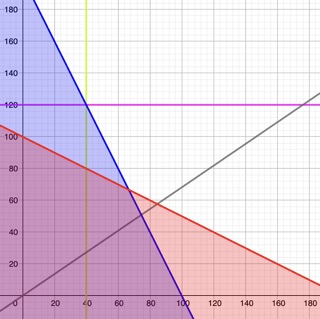
\includegraphics[scale=0.5]{es.jpeg}
\caption{Rappresentazione grafica esempio} 
\label{rge}
\end{figure}

	
	
% Implementazione in Python
\subsection{Implementazione in Python}

\begin{lstlisting}
import pulp as p

# 1. creazione del modello
model = p.LpProblem("ProductMix", p.LpMaximize)

# 2. definisco le variabili decisionall
x_A = p.LpVariable("x_A", cat="Continuous", lowBound=0)
x_B = p.LpVariable("x_B", cat="LpContinuous", lowBound=0)

# 3. definisco la funzione obiettivo in funzione delle variabili decisionali
model += 15 * x_A + 10 * x_B

# 4. definire i vincoli
model += 4 * x_A + 2 * x_B \leq 400
model += 2 * x_A + 4 * x_B \leq 400
model += x_A \leq 40
model += x_B \leq 120

# 5. ricolvere il problema
model.solve()

# print della soluzione
print("next week produce {} pallets of A".format(x_A.varValue))
print("next week produce {} pallets of B".format(x_B.varValue))
\end{lstlisting}


% Esercitazione
\subsection{Esercitazione}

\begin{enumerate}
	\item Massimizzare la f.o. $z = 8x_1 + 6x_2$, con i vincoli:
		\begin{itemize}
			\item $x_1 \leq 5$
			\item $x_2 \leq 7$
			\item $4x_1 + 3x_2 \leq 29$
			\item $x_1, x_2 \geq 0$
		\end{itemize}
		
		\begin{figure}[H]
		\centering
		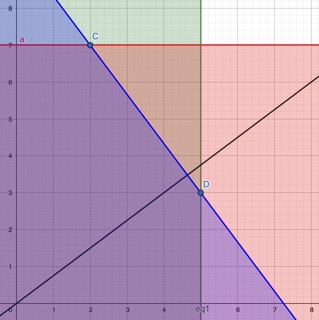
\includegraphics[scale=0.5]{es1.jpeg}
		\caption{Rappresentazione grafica esempio 1} 
		\label{rge1}
		\end{figure}
		
		$$\nabla z = \left[\begin{array}{c}
			\dfrac{dz}{dx_A}\\
			\dfrac{dz}{dx_B}
		\end{array}\right] = \left[\begin{array}{c}
			8\\
			6
		\end{array}\right]
		$$
		
		\hl{Abbiamo che esiste una curva di livello coincidente con lo spigolo CD, quindi abbiamo delle soluzioni ottime multiple}:
		\begin{itemize}
			\item vertice C, prendiamo allora vincolo 2 e 3:
				$$x_2 = 7 \to x_1 = 2$$
			
			\item vertice D, prendiamo allora vincolo 1 e 3:
				$$x_1 = 5 \to x_2 = 3$$
		
			\item punti del segmento CD
		\end{itemize}
		
		Quindi $z = 58$
	
	
	\item Minimizziamo la f.o. $z = 25x_1 + 22x_2$, con i vincoli:
		\begin{itemize}
			\item $x_1 + x_2 \geq 5$
			\item $3x_1 + 2x_2 \geq 12$
			\item $3x_1 + 6x_2 \geq 18$
			\item $x_1, x_2 \geq 0$
		\end{itemize}
		
		\begin{figure}[H]
		\centering
		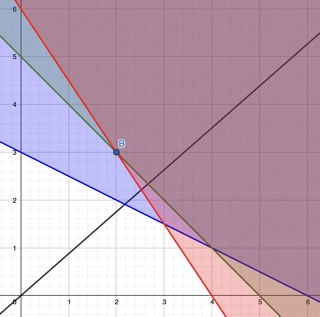
\includegraphics[scale=0.5]{es2.jpeg}
		\caption{Rappresentazione grafica esempio 2} 
		\label{rge2}
		\end{figure}
		
		$$\nabla z = \left[\begin{array}{c}
			\dfrac{dz}{dx_A}\\
			\dfrac{dz}{dx_B}
		\end{array}\right] = \left[\begin{array}{c}
			25\\
			22
		\end{array}\right]
		$$
		
		Per poter minimizzare, tracciando la curva di livello, trovando che la soluzione ottima si troverà dal punto B dato dall'intersezione dei vincoli 1 e 2:
		$$x_1 = 2, x_2 = 3$$
		
		Quindi $z= 116$
		
	\item Massimizziamo la f.o. $z = 2x_1 + x_2$, con i vincoli:
		\begin{itemize}
			\item $x_1 - x_2 \leq 1$
			\item $2x_1 + x_2 \geq 6$
			\item $x_2 \geq 6$
			\item $x_1, x_2 \geq 0$
		\end{itemize}
		
		\begin{figure}[H]
		\centering
		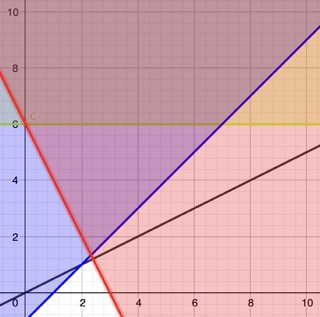
\includegraphics[scale=0.5]{es3.jpeg}
		\caption{Rappresentazione grafica esempio 3} 
		\label{rge3}
		\end{figure}
		
		$$\nabla z = \left[\begin{array}{c}
			\dfrac{dz}{dx_A}\\
			\dfrac{dz}{dx_B}
		\end{array}\right] = \left[\begin{array}{c}
			2\\
			1
		\end{array}\right]
		$$
		
		\hl{Non raggiungeremo la regione ammissibile, quindi il problema non ammette una soluzione ottima}.
		
	\item Minimizziamo la f.o. $z = -2x_1 + 3x_2$, con i vincoli:
		\begin{itemize}
			\item $x_1 - 2x_2 \geq -2$
			\item $2x_1 - x_2 \leq 3$
			\item $x_2 \geq 4$
			\item $x_1, x_2 \geq 0$
		\end{itemize}
		
		\begin{figure}[H]
		\centering
		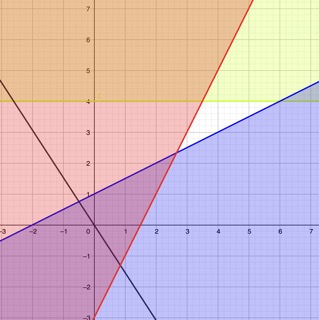
\includegraphics[scale=0.5]{es4.jpeg}
		\caption{Rappresentazione grafica esempio 4} 
		\label{rge4}
		\end{figure}

		
		$$\nabla z = \left[\begin{array}{c}
			\dfrac{dz}{dx_A}\\
			\dfrac{dz}{dx_B}
		\end{array}\right] = \left[\begin{array}{c}
			-2\\
			3
		\end{array}\right]
		$$
		
		\hl{La regione ammissibile e' vuota e per tanto i problema e' inammissibile, quindi non esiste un punto che soddisfa contemporaneamente tutti i vincoli}.
		
	\item L'azienda vuole decide oltre al piano di produzione anche la giusta riallocazione degli addetti (10-10) tra i due reparti.		
		Le variabili decisionali sono:
		\begin{itemize}
			\item $x_A, x_B$: i prodotti
			\item $n_p$: \# addetti allocati al reparto produzione
			\item $n_a$: \#addetti allocati al reparto assemblaggio
		\end{itemize}
		
		Quindi andremo ad aggiungere il vincolo per cui $n_p + n_a = 20$.
		
		Perciò avremo: $z = 15x_A + 10x_B$, con vincoli:
		\begin{itemize}
			\item $4x_A + 2x_B \leq 40n_p$
			\item $2x_A + 4x_B \leq 40n_a$
			\item $x_A \leq 40$
			\item $x_B \leq 120$
			\item $n_a + n_p = 20$
			\item $x_A, x_B, n_a, n_p \geq 0$
		\end{itemize}
		

\end{enumerate}







